\documentclass[aspectratio=169,10pt]{beamer}

\usepackage{iftex}
\ifPDFTeX
  \PackageError{surf-bms-deck}{This deck uses Liberation Sans through fontspec}{Build with Tectonic or XeLaTeX}
\else
  \usepackage{fontspec}
  \defaultfontfeatures{Ligatures=TeX,Scale=MatchLowercase}
  \setsansfont{LiberationSans-Regular.ttf}[
    Path=fonts/,
    BoldFont=LiberationSans-Bold.ttf,
    ItalicFont=LiberationSans-Italic.ttf,
    BoldItalicFont=LiberationSans-BoldItalic.ttf
  ]
  \setmainfont{LiberationSans-Regular.ttf}[
    Path=fonts/,
    BoldFont=LiberationSans-Bold.ttf,
    ItalicFont=LiberationSans-Italic.ttf,
    BoldItalicFont=LiberationSans-BoldItalic.ttf
  ]
\fi

\usepackage{array,booktabs,tabularx}
\usepackage{graphicx}
\usepackage{tikz}
\usetikzlibrary{calc,positioning}
\usepackage{hyperref}

% Slide text stays ragged and unhyphenated for clean projected reading.
\hyphenpenalty=10000
\exhyphenpenalty=10000
\pretolerance=10000
\tolerance=2000
\emergencystretch=1.2em

% Palette B: the DUNE identity colors with accessible editorial ink tones.
\definecolor{DuneBlue}{HTML}{7CAED5}
\definecolor{DuneOrange}{HTML}{F2682B}
\definecolor{DuneDeepBlue}{HTML}{3E6178}
\definecolor{DuneDeepBlueInk}{HTML}{304E62}
\definecolor{DuneInk}{HTML}{1C2834}
\definecolor{DuneSecondary}{HTML}{596875}
\definecolor{DuneRule}{HTML}{8996A0}
\definecolor{DuneLightRule}{HTML}{DCE3E7}
\definecolor{DuneBlueTint}{HTML}{E5EFF7}
\definecolor{DuneOrangeTint}{HTML}{FCE1D5}
\definecolor{DuneCanvas}{HTML}{F7F8FA}
\definecolor{DuneWhite}{HTML}{FFFFFF}

\hypersetup{
  colorlinks=true,
  linkcolor=DuneDeepBlueInk,
  urlcolor=DuneDeepBlueInk,
  pdftitle={SURF facility status and DUNE response},
  pdfauthor={DUNE Far Detector}
}

\setbeamercolor{normal text}{fg=DuneInk,bg=DuneCanvas}
\setbeamercolor{frametitle}{fg=DuneInk,bg=DuneCanvas}
\setbeamercolor{structure}{fg=DuneDeepBlueInk}
\setbeamercolor{surface}{fg=DuneInk,bg=DuneWhite}
\setbeamercolor{soft surface}{fg=DuneInk,bg=DuneBlueTint}
\setbeamercolor{warm surface}{fg=DuneInk,bg=DuneOrangeTint}
\setbeamerfont{normal text}{size=\small}
\setbeamerfont{frametitle}{size=\fontsize{20}{23}\selectfont,series=\bfseries}
\setbeamertemplate{navigation symbols}{}
\setbeamertemplate{headline}{}
\setbeamertemplate{footline}{}
\setbeamersize{text margin left=0.82cm,text margin right=0.82cm}

\newcommand{\decklabel}{DUNE FAR DETECTOR \textperiodcentered{} SURF FACILITY INTERFACE}

\newcommand{\editorialbackground}{%
  \begin{tikzpicture}[remember picture,overlay]
    \fill[DuneCanvas] (current page.south west) rectangle (current page.north east);
    \fill[DuneBlue] (current page.north west) rectangle
      ($(current page.north east)+(0,-0.07)$);
    \fill[DuneOrange] ($(current page.north west)+(0.82,-0.07)$) rectangle ++(1.45,-0.035);
    \node[anchor=north west,text=DuneSecondary,font=\fontsize{5.8}{7}\selectfont\bfseries]
      at ($(current page.north west)+(0.82,-0.22)$) {\decklabel};
    \node[anchor=north east,text=DuneDeepBlueInk,font=\fontsize{6.2}{7}\selectfont\bfseries]
      at ($(current page.north east)+(-0.82,-0.22)$) {\insertframenumber};
    \draw[DuneLightRule,line width=0.45pt]
      ($(current page.south west)+(0.82,0.42)$) --
      ($(current page.south east)+(-0.82,0.42)$);
  \end{tikzpicture}%
}
\setbeamertemplate{background canvas}{\editorialbackground}

\setbeamertemplate{frametitle}{%
  \vspace*{0.46cm}%
  \nointerlineskip
  \begin{beamercolorbox}[wd=\textwidth,sep=0pt]{frametitle}
    \usebeamerfont{frametitle}\insertframetitle\strut
  \end{beamercolorbox}%
  \vspace{0.05cm}%
  {\color{DuneOrange}\rule{1.45cm}{1.35pt}\par}%
  \vspace{0.03cm}%
}

\newcommand{\statement}[1]{%
  \begin{tikzpicture}
    \node[
      anchor=north west,
      draw=DuneLightRule,
      fill=DuneWhite,
      rounded corners=3pt,
      line width=0.45pt,
      text width=\dimexpr\textwidth-20pt\relax,
      inner xsep=8pt,
      inner ysep=5pt,
      outer sep=0pt,
      align=left,
      font=\fontsize{12}{14.5}\selectfont\bfseries,
      text=DuneDeepBlueInk
    ] (statementbox) at (0,0) {#1};
    \draw[DuneBlue,line width=2.5pt]
      (statementbox.north west) -- (statementbox.south west);
  \end{tikzpicture}%
}

\newcommand{\infocard}[5][1.82cm]{%
  \begin{tikzpicture}
    \node[
      anchor=north west,
      draw=DuneLightRule,
      fill=DuneWhite,
      rounded corners=3pt,
      line width=0.45pt,
      text width=\dimexpr\linewidth-20pt\relax,
      minimum height=#1,
      inner xsep=7pt,
      inner ysep=5pt,
      outer sep=0pt,
      align=left
    ] (card) at (0,0) {%
      {\color{#2}\fontsize{6.4}{7.4}\selectfont\bfseries\MakeUppercase{#3}\par}
      \vspace{0.7mm}
      {\color{DuneInk}\fontsize{9.8}{11.5}\selectfont\bfseries #4\par}
      \vspace{0.45mm}
      {\color{DuneSecondary}\fontsize{7.7}{9.2}\selectfont #5\par}
    };
    \draw[#2,line width=2.1pt] (card.north west) -- (card.north east);
  \end{tikzpicture}%
}

\newcommand{\diagrambackground}{%
  \begin{tikzpicture}[remember picture,overlay]
    \fill[DuneWhite] (current page.south west) rectangle (current page.north east);
  \end{tikzpicture}%
}

\title{SURF facility status and DUNE response}
\author{DUNE Far Detector}

\begin{document}

% 1 — Title
{
\setbeamertemplate{background canvas}{%
  \begin{tikzpicture}[remember picture,overlay]
    \fill[DuneCanvas] (current page.south west) rectangle (current page.north east);
    \fill[DuneBlue] (current page.north west) rectangle
      ($(current page.north east)+(0,-0.10)$);
    \fill[DuneOrange] ($(current page.north west)+(0.92,-0.10)$) rectangle ++(2.1,-0.055);
    \fill[DuneBlueTint] ($(current page.north east)+(-4.5,0)$) rectangle
      ($(current page.south east)+(0,0)$);
  \end{tikzpicture}%
}
\begin{frame}[plain,noframenumbering]
  \begin{tikzpicture}[remember picture,overlay]
    \node[anchor=north east]
      at ($(current page.north east)+(-0.76,-0.72)$)
      {
\includegraphics[width=3.05cm]{logos/DUNElogo_color.png}};
    \node[
      anchor=north west,
      text=DuneSecondary,
      font=\fontsize{7}{8}\selectfont\bfseries
    ] at ($(current page.north west)+(0.94,-0.68)$)
      {FAR DETECTOR \textperiodcentered{} SANFORD UNDERGROUND RESEARCH FACILITY};
    \node[
      anchor=north west,
      text width=10.7cm,
      text=DuneInk,
      align=left,
      font=\fontsize{29}{32}\selectfont\bfseries
    ] at ($(current page.north west)+(0.92,-1.48)$)
      {SURF facility status\\and DUNE response};
    \node[
      anchor=north west,
      text width=10.5cm,
      text=DuneSecondary,
      align=left,
      font=\fontsize{13}{17}\selectfont
    ] at ($(current page.north west)+(0.94,-3.92)$)
      {A reference architecture for monitoring, orderly DAQ shutdown, detector protection, and local protection};
    \node[
      anchor=north west,
      draw=DuneLightRule,
      fill=DuneWhite,
      rounded corners=4pt,
      line width=0.5pt,
      text width=10.15cm,
      inner sep=11pt,
      text=DuneDeepBlueInk,
      align=left,
      font=\fontsize{12.5}{16}\selectfont\bfseries
    ] (titlemessage) at ($(current page.north west)+(0.94,-5.58)$)
      {Facility information provides context. Action authority stays with the system that owns the response.};
    \draw[DuneOrange,line width=3pt]
      (titlemessage.north west) -- (titlemessage.south west);
  \end{tikzpicture}
\end{frame}
}

% 2 — Why the interface matters
\begin{frame}[t]{Why the interface matters}
  \statement{Underground operations depend on facility conditions, while the experiment and the facility retain separate control authority.}
  \vspace{1.6mm}
  \begin{columns}[T,totalwidth=\textwidth]
    \begin{column}{0.492\textwidth}
      \infocard{DuneDeepBlue}{Operational continuity}{Power and reserve}{Loss of normal power can limit the time available for an orderly DAQ stop.}
      \vspace{1.2mm}
      \infocard{DuneInk}{Source authority}{Fire and air}{SURF owns fire, low-oxygen, and ventilation alarms and the personnel response.}
    \end{column}
    \begin{column}{0.492\textwidth}
      \infocard{DuneOrange}{Approved response}{Cryogenics, cooling, and water}{DUNE action follows an approved cause and effect owned by the source and detector systems.}
      \vspace{1.2mm}
      \infocard{DuneSecondary}{Operating context}{Network, weather, and access}{These conditions inform operations. A lost information path remains visible.}
    \end{column}
  \end{columns}
\end{frame}

% 3 — Four functions
\begin{frame}[t]{Four functions remain distinct}
  \statement{The same facility event can appear on several paths without giving those paths the same authority.}
  \vspace{1.6mm}
  \begin{columns}[T,totalwidth=\textwidth]
    \begin{column}{0.492\textwidth}
      \infocard{DuneBlue}{Context}{Facility monitoring}{Source $\rightarrow$ BMS $\rightarrow$ boundary $\rightarrow$ Slow Controls. The source owner retains alarm and reset authority.}
      \vspace{1.2mm}
      \infocard{DuneInk}{Approved action}{Detector protection}{Approved source $\rightarrow$ open interface $\rightarrow$ DPS. DPS owns permit, inhibit, trip, latch, and reset.}
    \end{column}
    \begin{column}{0.492\textwidth}
      \infocard{DuneOrange}{Operational action}{Orderly DAQ shutdown}{UPS state $\rightarrow$ backed automation $\rightarrow$ Run Control. DAQ owns run state; this path carries no protection credit.}
      \vspace{1.2mm}
      \infocard{DuneDeepBlue}{At the load}{Local protection}{Local sensor $\rightarrow$ local logic $\rightarrow$ affected load. The equipment owner retains action and restart authority.}
    \end{column}
  \end{columns}
\end{frame}

% 4 — Reference architecture
{
\setbeamertemplate{background canvas}{\diagrambackground}
\begin{frame}[plain]
  \begin{tikzpicture}[remember picture,overlay]
    \node[anchor=center,inner sep=0pt] at (current page.center)
      {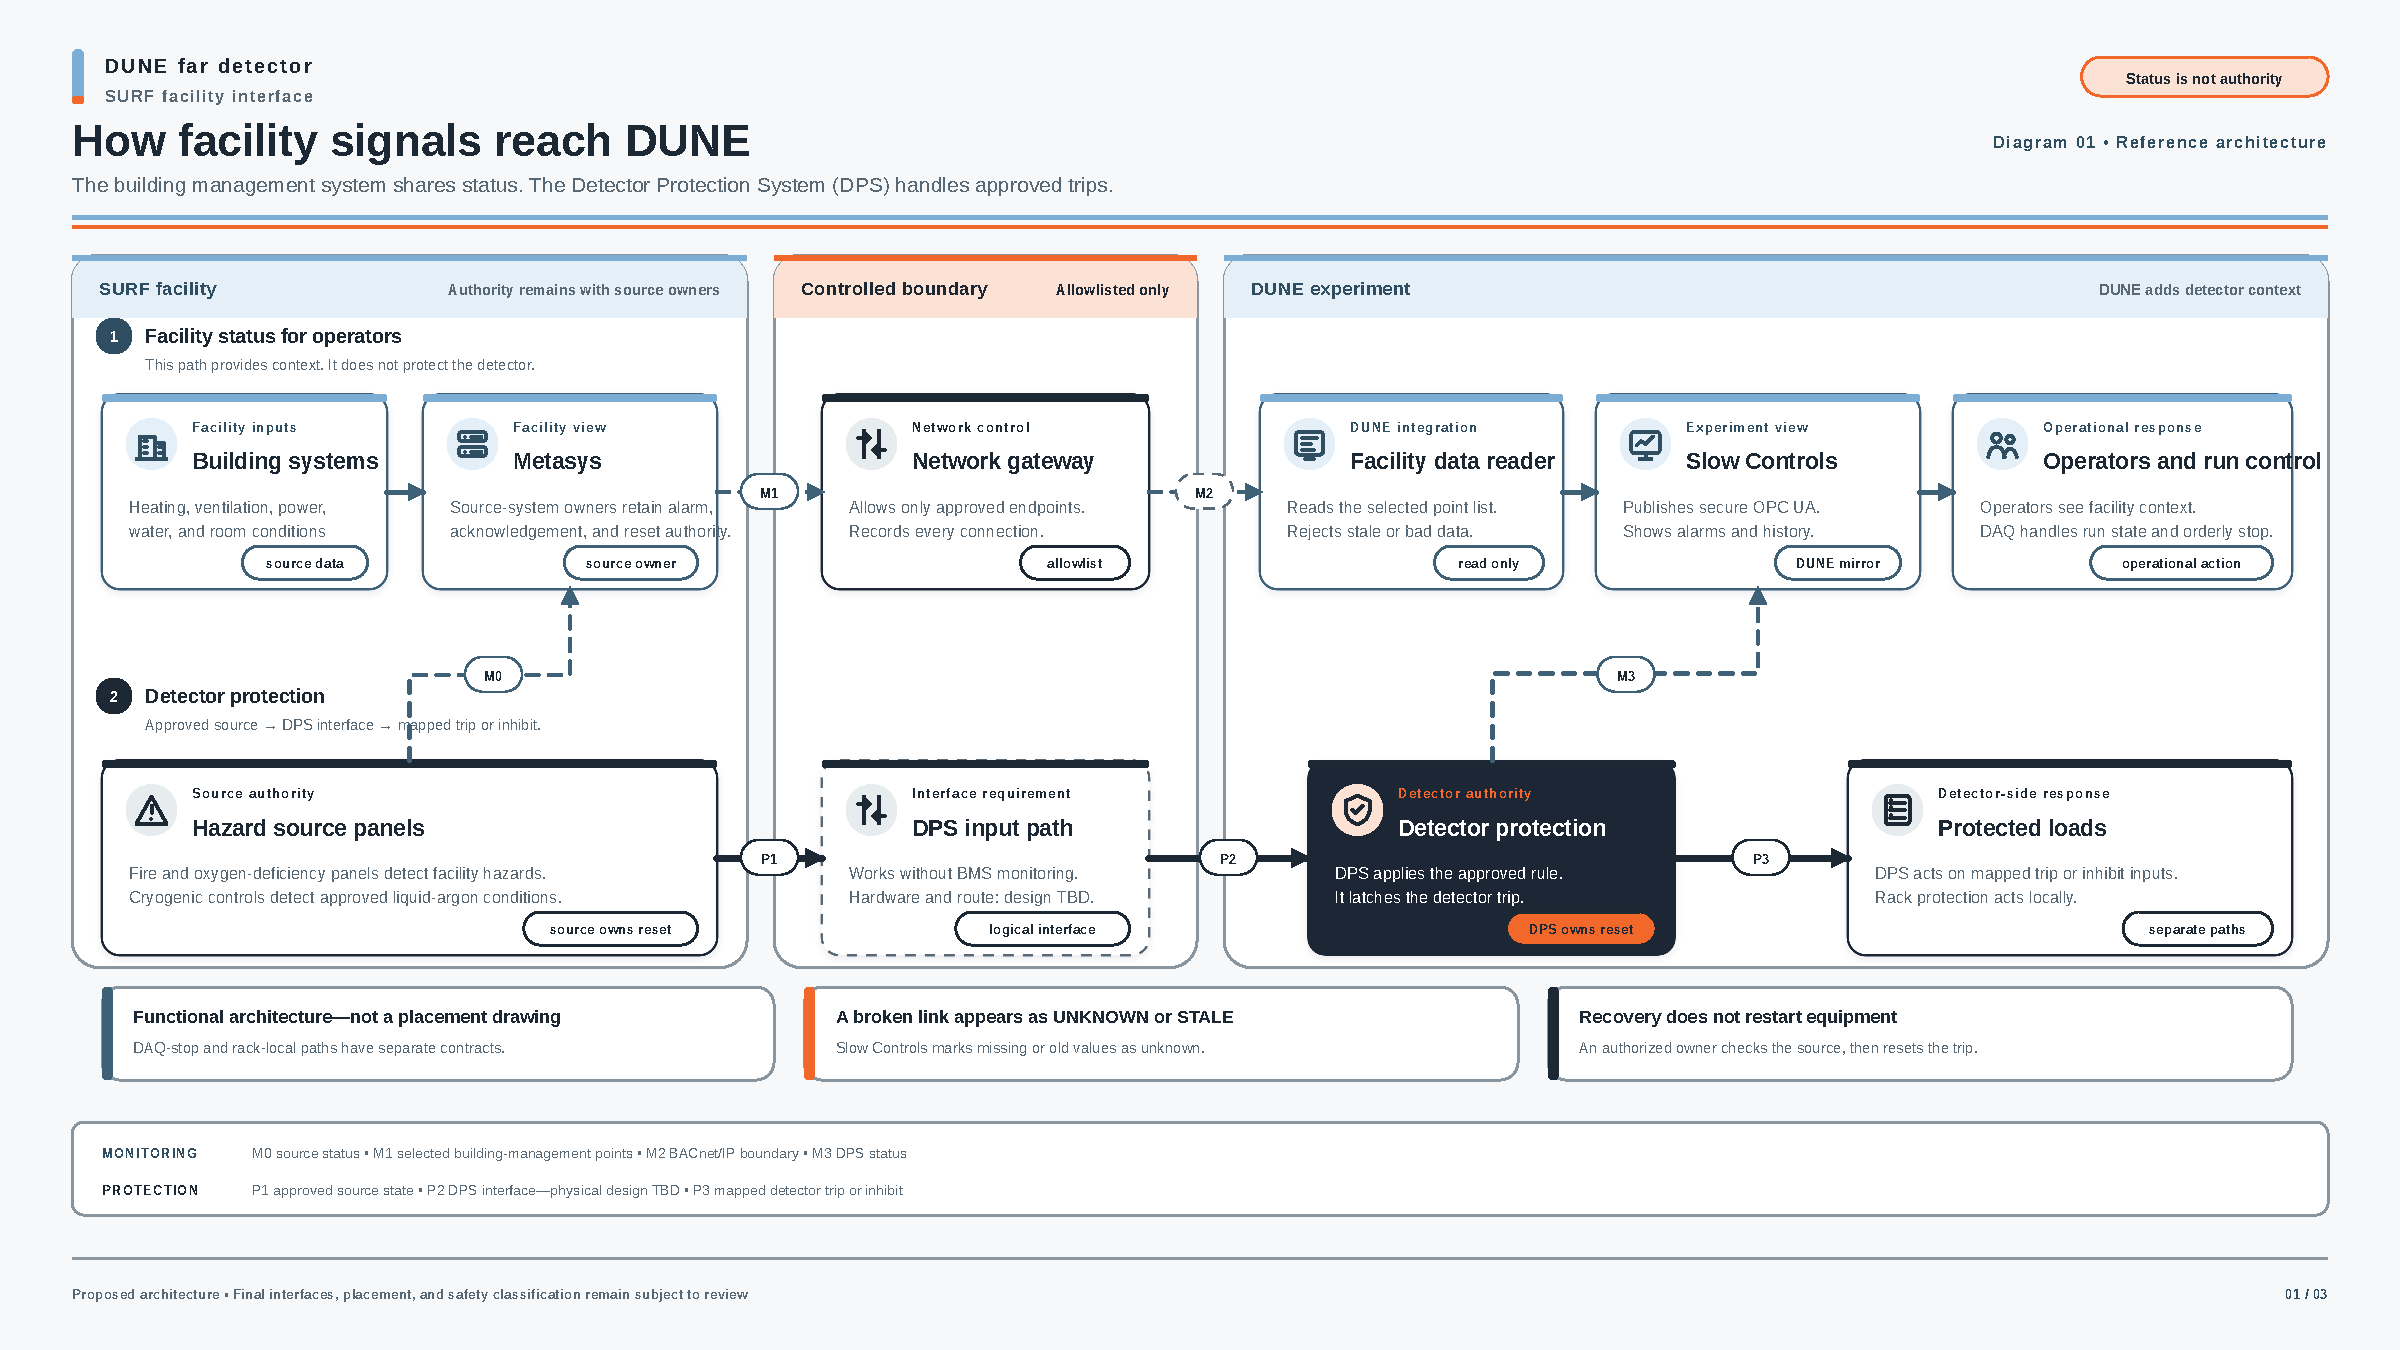
\includegraphics[width=0.96\paperwidth,height=0.96\paperheight,keepaspectratio]{figures/01_bms_dcs_dps_boundary.pdf}};
  \end{tikzpicture}
\end{frame}
}

% 5 — Alarm authority
{
\setbeamertemplate{background canvas}{\diagrambackground}
\begin{frame}[plain]
  \begin{tikzpicture}[remember picture,overlay]
    \node[anchor=center,inner sep=0pt] at (current page.center)
      {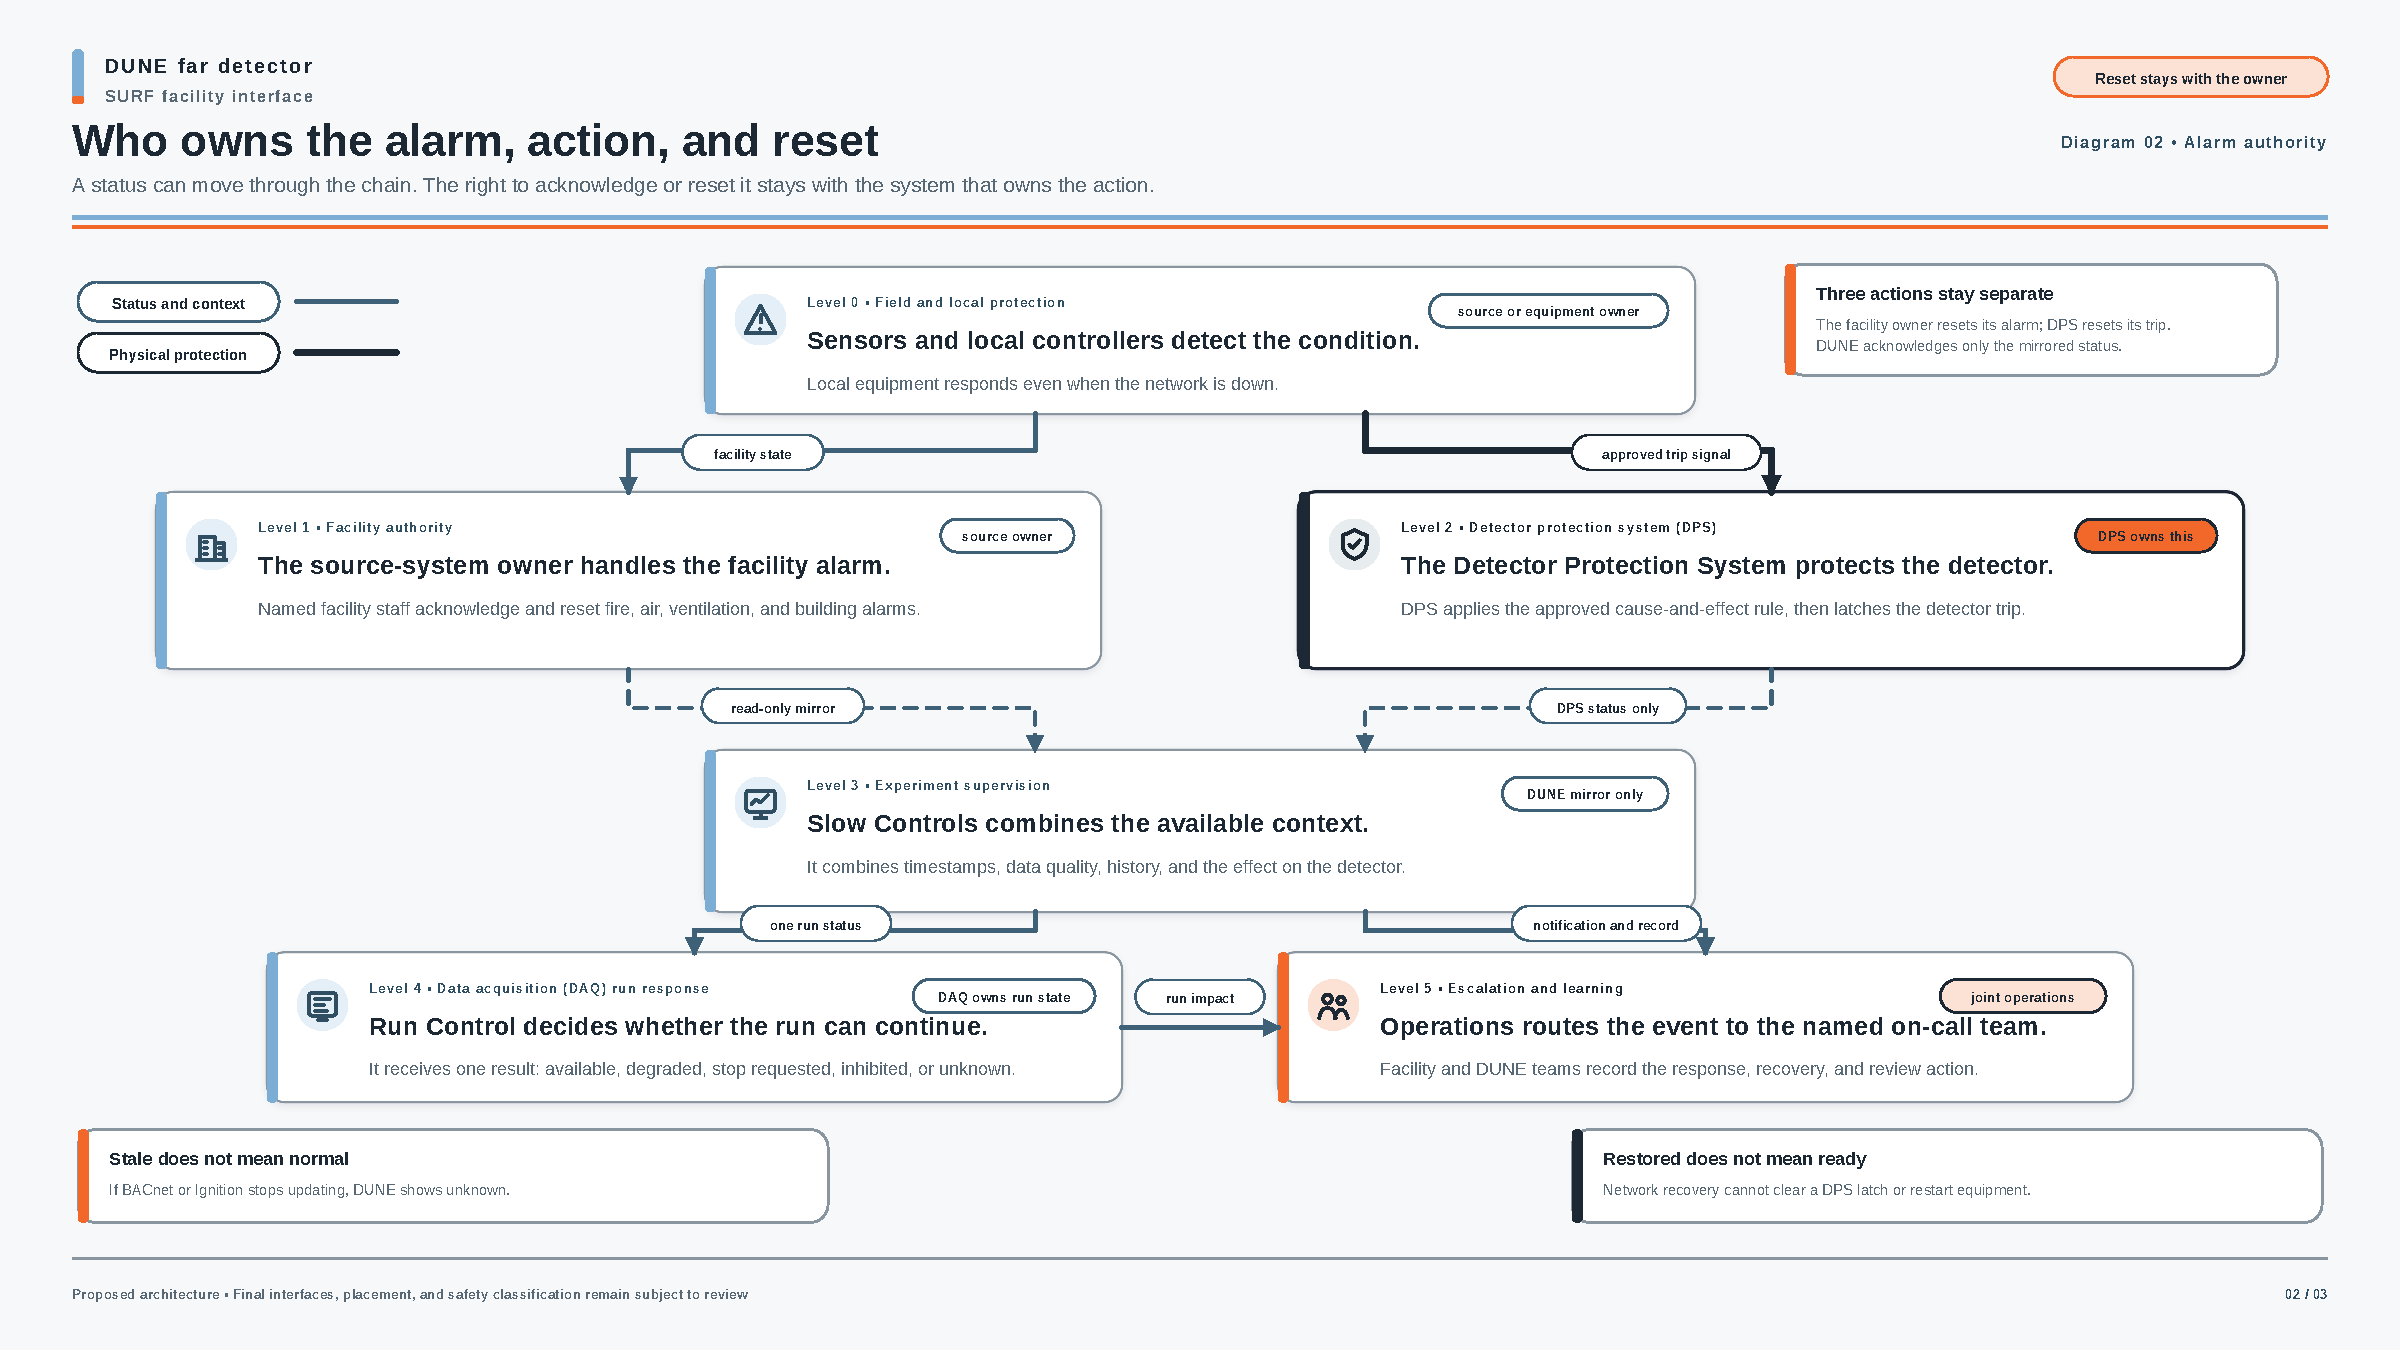
\includegraphics[width=0.96\paperwidth,height=0.96\paperheight,keepaspectratio]{figures/02_alarm_authority_hierarchy.pdf}};
  \end{tikzpicture}
\end{frame}
}

% 6 — Information crossing the boundary
\begin{frame}[t]{What crosses the boundary}
  \statement{DUNE receives facility state, not authority over the source alarm or reset.}
  \vspace{1.6mm}
  \begin{columns}[T,totalwidth=\textwidth]
    \begin{column}{0.492\textwidth}
      \infocard{DuneDeepBlue}{Facility status}{BACnet/IP}{Selected source points carry value, state, source time, quality, and freshness.}
      \vspace{1.2mm}
      \infocard{DuneBlue}{DUNE view}{OPC UA}{Stable tags add units, age, detector context, alarms, and history.}
    \end{column}
    \begin{column}{0.492\textwidth}
      \infocard{DuneOrange}{Service health}{SNMPv3}{Telemetry exposes network health and the health of backed services.}
      \vspace{1.2mm}
      \infocard{DuneSecondary}{Event chronology}{NTP and protected logs}{Source time and receive time support a coherent account of an event.}
    \end{column}
  \end{columns}
\end{frame}

% 7 — Failure response
{
\setbeamertemplate{background canvas}{\diagrambackground}
\begin{frame}[plain]
  \begin{tikzpicture}[remember picture,overlay]
    \node[anchor=center,inner sep=0pt] at (current page.center)
      {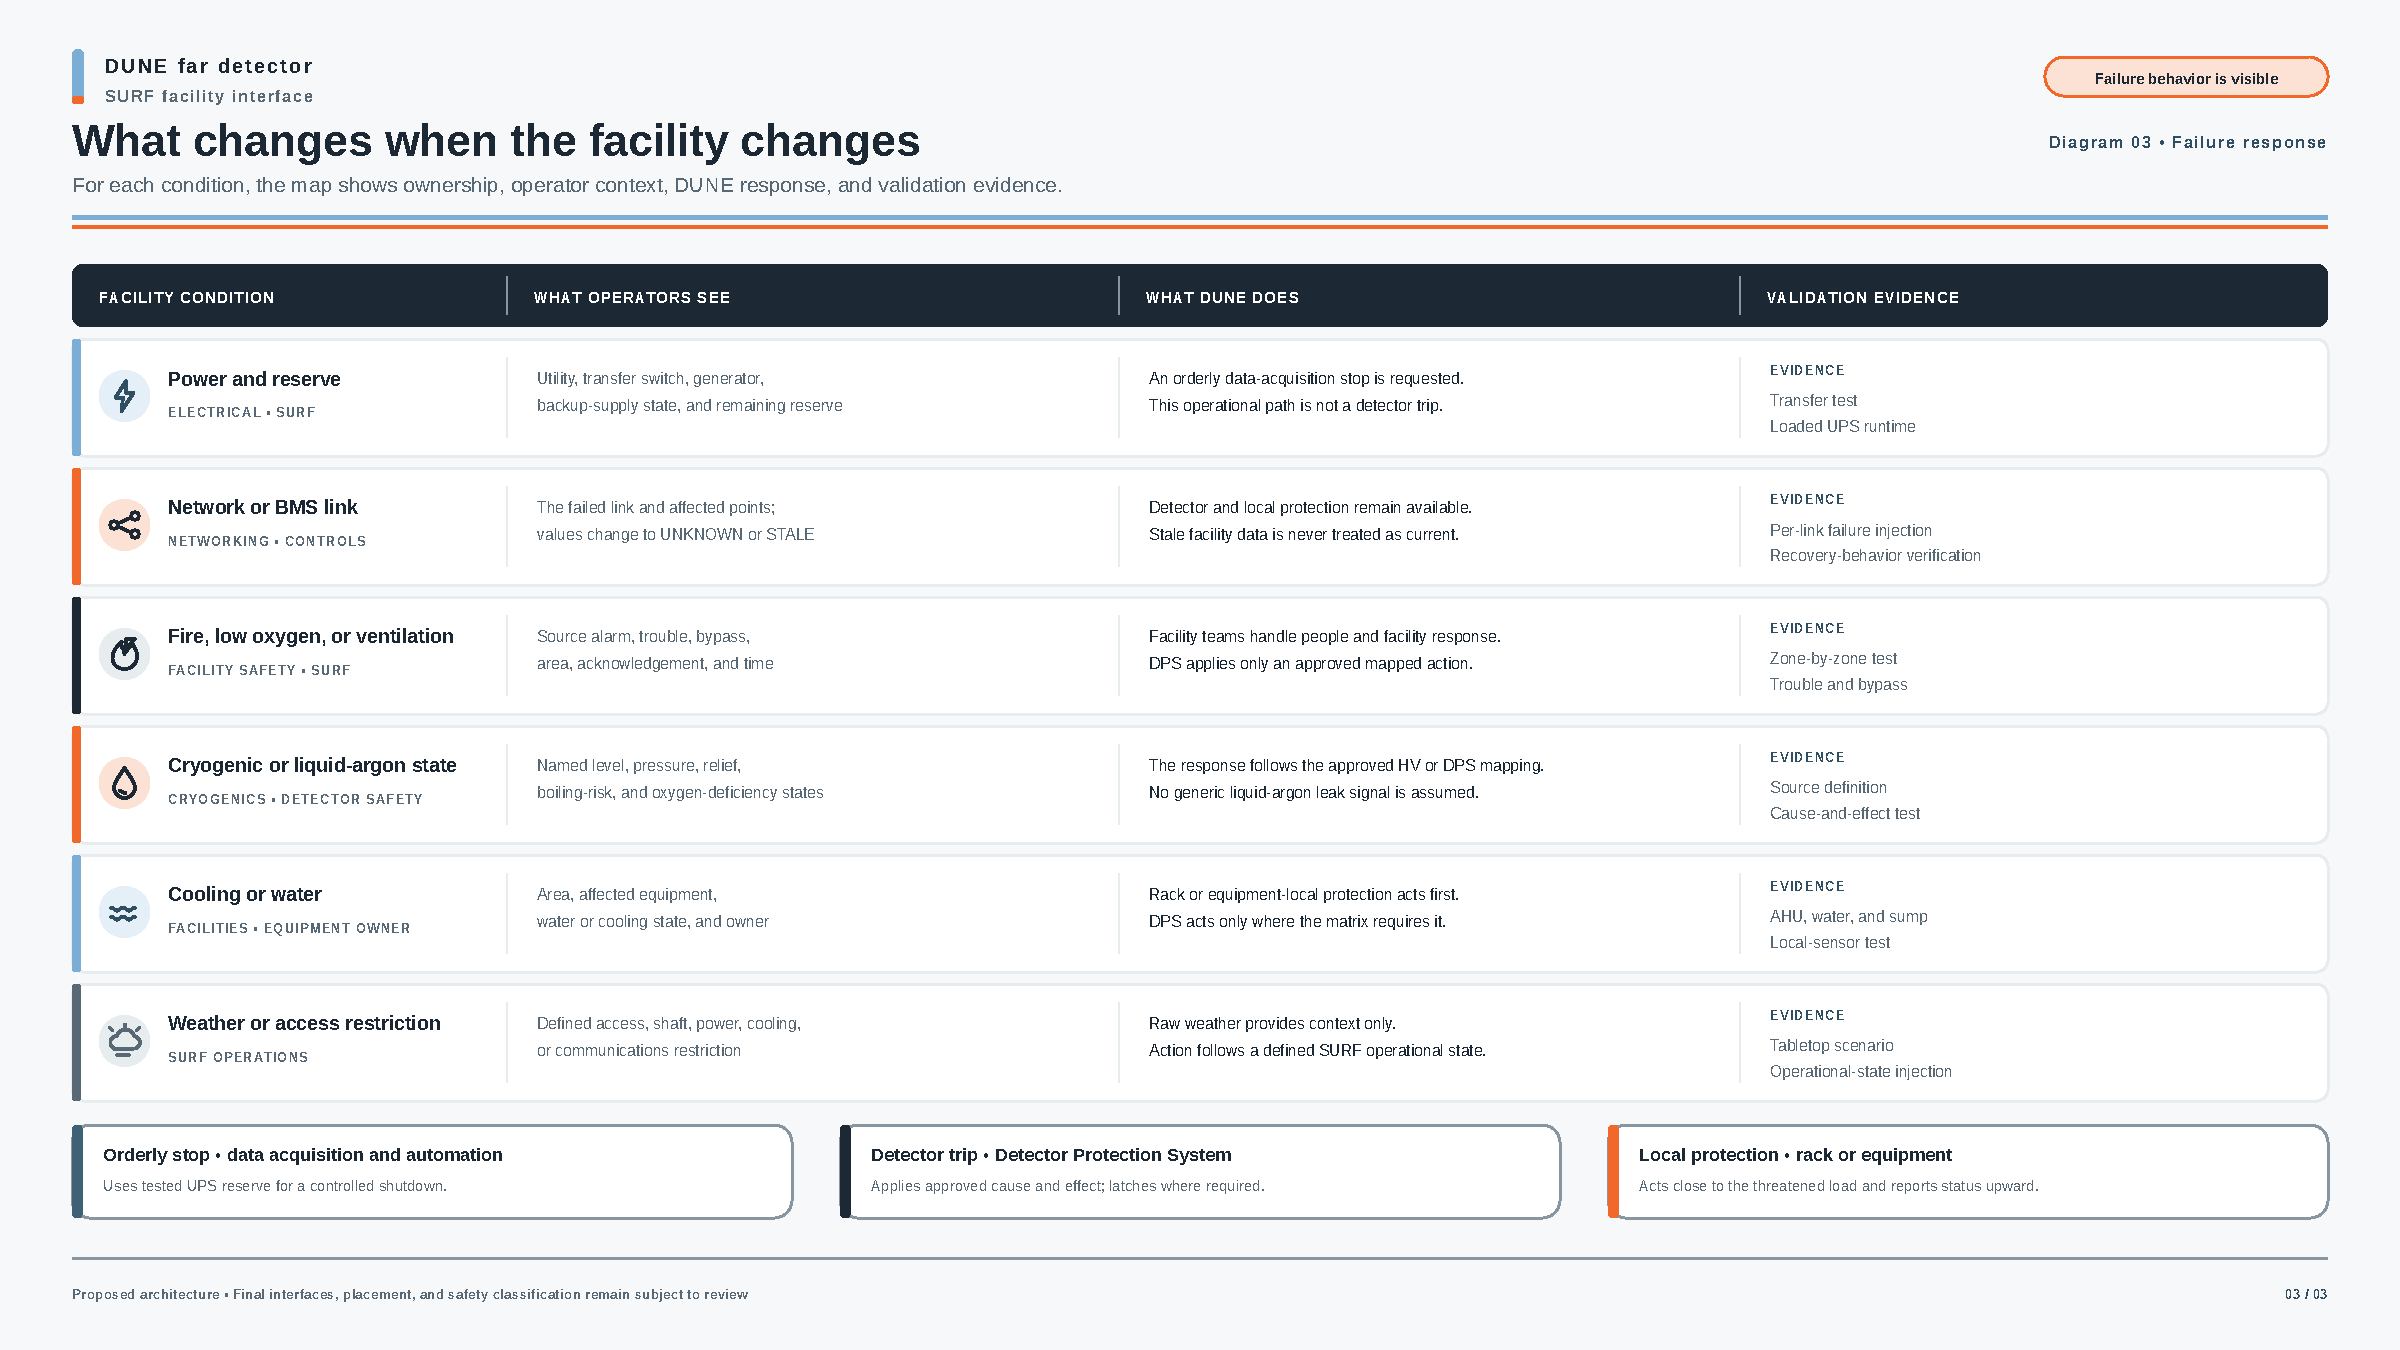
\includegraphics[width=0.96\paperwidth,height=0.96\paperheight,keepaspectratio]{figures/03_failure_response_map.pdf}};
  \end{tikzpicture}
\end{frame}
}

% 8 — Unavailable information
\begin{frame}[t]{Unavailable information stays visible}
  \statement{A failed data path changes what DUNE knows; it does not change the source condition or authorize a restart.}
  \vspace{1.6mm}
  \begin{columns}[T,totalwidth=\textwidth]
    \begin{column}{0.492\textwidth}
      \infocard{DuneBlue}{GOOD}{Current}{The value is current and carries valid source, time, and quality information.}
      \vspace{1.2mm}
      \infocard{DuneOrange}{STALE}{Aging}{The value remains historical context while its age and alarm stay visible.}
    \end{column}
    \begin{column}{0.492\textwidth}
      \infocard{DuneInk}{UNKNOWN}{Absent}{The source, link, or service cannot provide a trustworthy current state.}
      \vspace{1.2mm}
      \infocard{DuneDeepBlue}{RECOVERY}{Restored}{Updates resume while latches, inspection, and restart authority stay with their owners.}
    \end{column}
  \end{columns}
\end{frame}

% 9 — Starting points and open questions
\begin{frame}[t]{What is established—and what remains open}
  \statement{The functional boundary is clear; its remaining interface facts belong with named owners.}
  \vspace{1.7mm}
  \begin{beamercolorbox}[wd=\textwidth,sep=0pt,rounded=true]{surface}
    \vspace{7pt}\hspace{8pt}%
    \begin{minipage}{\dimexpr\textwidth-16pt\relax}
      \fontsize{8}{9.8}\selectfont
      \renewcommand{\arraystretch}{1.18}
      \begin{tabularx}{\linewidth}{@{}>{\raggedright\arraybackslash}p{0.44\linewidth}>{\raggedright\arraybackslash}X@{}}
        {\color{DuneDeepBlueInk}\fontsize{7}{8}\selectfont\bfseries ESTABLISHED STARTING POINT} &
        {\color{DuneOrange}\fontsize{7}{8}\selectfont\bfseries OPEN ARCHITECTURE QUESTION} \\
        \midrule
        {\bfseries SURF retains source-alarm authority.} & Authoritative points and state definitions. \\
        {\bfseries The BMS-to-DUNE path is monitoring only.} & Live service boundary, security behavior, and ownership. \\
        {\bfseries DAQ, DPS, and local action remain separate.} & Conditions for an orderly stop or detector action. \\
        {\bfseries The diagrams define functions, not equipment.} & Interface medium, supervision, and failure behavior. \\
      \end{tabularx}
    \end{minipage}
    \vspace{7pt}
  \end{beamercolorbox}
\end{frame}

% 10 — Architecture acceptance
\begin{frame}[t]{Architecture acceptance}
  \statement{Acceptance connects four properties: authority, information, failure behavior, and verification.}
  \vspace{1.6mm}
  \begin{columns}[T,totalwidth=\textwidth]
    \begin{column}{0.492\textwidth}
      \infocard{DuneInk}{Acceptance dimension}{Authority}{One owner is identifiable for the source alarm, run state, detector action, and local action.}
      \vspace{1.2mm}
      \infocard{DuneBlue}{Acceptance dimension}{Information}{Source, time, quality, age, and state meaning remain intact from origin to operator view.}
    \end{column}
    \begin{column}{0.492\textwidth}
      \infocard{DuneOrange}{Acceptance dimension}{Failure behavior}{Lost or stale data is visible; monitoring loss does not remove detector or local protection.}
      \vspace{1.2mm}
      \infocard{DuneDeepBlue}{Acceptance dimension}{Verification}{Test evidence covers the boundary, selectivity, loss, and recovery behavior.}
    \end{column}
  \end{columns}
\end{frame}

\end{document}
